\documentclass[a4paper, 13pt]{article}
\usepackage{vntex}
\usepackage[dvipsnames]{xcolor}
%\usepackage[english,vietnam]{babel}
%\usepackage[utf8]{inputenc}

%\usepackage[utf8]{inputenc}
%\usepackage[francais]{babel}
\usepackage{a4wide,amssymb,epsfig,latexsym,array,hhline,fancyhdr}
\usepackage[normalem]{ulem}
%\usepackage{soul}
\usepackage{colortbl}
\usepackage{longtable}
\usepackage[makeroom]{cancel}
\usepackage{amsmath}
\usepackage{amsfonts}
\usepackage{amssymb}
\usepackage{amsthm}
\usepackage{multicol,longtable,amscd}
\usepackage{diagbox}%Make diagonal lines in tables
\usepackage{booktabs}
\usepackage{alltt}
\usepackage[framemethod=tikz]{mdframed}% For highlighting paragraph backgrounds
\usepackage{caption,subcaption}
\usepackage{listings}
\usepackage{color}
\usepackage{lastpage}
\usepackage[lined,boxed,commentsnumbered]{algorithm2e}
\usepackage{enumerate}
\usepackage{color}
\usepackage{graphicx}							% Standard graphics package
\usepackage{array}
\usepackage{tabularx, caption}
\usepackage{multirow}
\usepackage{multicol}
\usepackage{rotating}
\usepackage{graphics}
\usepackage{geometry}
\usepackage{setspace}
\usepackage{epsfig}
\usepackage{tikz , pgf}
\usetikzlibrary{arrows,snakes,backgrounds}
\usepackage[unicode]{hyperref}
\hypersetup{urlcolor=blue,linkcolor=black,citecolor=black,colorlinks=true} 
%\usepackage{pstcol} 								% PSTricks with the standard color package
\definecolor{bblue}{RGB}{239,239,255}
\colorlet{mygray}{black!30}
\colorlet{mygreen}{green!60!blue}
\colorlet{mymauve}{red!60!blue}

\newtheorem{theorem}{{\bf Định lý}}
\newtheorem{property}{{\bf Tính chất}}
\newtheorem{proposition}{{\bf Mệnh đề}}
\newtheorem{corollary}[proposition]{{\bf Hệ quả}}
\newtheorem{lemma}[proposition]{{\bf Bổ đề}}
\theoremstyle{definition}
\newtheorem{exer}{Bài toán}

\def\thesislayout{	% A4: 210 × 297
	\geometry{
		a4paper,
		total={160mm,240mm},  % fix over page
		left=25mm,
		top=40mm,
        bottom=40mm,
	}
}


\thesislayout
\lstdefinelanguage{JavaScript}{
  keywords={typeof, new, true, false, catch, function, return, null, catch, switch, var, if, in, while, do, else, case, break, import, const, let, from},
  keywordstyle=\color{blue}\bfseries,
  ndkeywords={class, export, boolean, throw, implements, import, this},
  ndkeywordstyle=\color{darkgray}\bfseries,
  identifierstyle=\color{black},
  sensitive=false,
  comment=[l]{//},
  morecomment=[s]{/*}{*/},
  commentstyle=\color{purple}\ttfamily,
  stringstyle=\color{red}\ttfamily,
  morestring=[b]',
  morestring=[b]"
}

\lstset{
  backgroundcolor=\color{gray!10},  
  basicstyle=\ttfamily,
  columns=fullflexible,
  breakatwhitespace=false,      
  breaklines=true,                
  captionpos=b,                    
  commentstyle=\color{mygreen}, 
  extendedchars=true,              
  frame=single,                   
  keepspaces=true,             
  keywordstyle=\color{blue},
  language = JavaScript,
  numbers=none,                
  numbersep=5pt,                   
  numberstyle=\tiny\color{blue}, 
  rulecolor=\color{mygray},        
  showspaces=false,               
  showtabs=false,                 
  stepnumber=5,                  
  stringstyle=\color{mymauve},    
  tabsize=3,                      
  title=\lstname                
}

%\usepackage{fancyhdr}
\setlength{\headheight}{40pt}
\pagestyle{fancy}
\fancyhead{} % clear all header fields
\fancyhead[L]{
 \begin{tabular}{rl}
    \begin{picture}(20,15)(0,0)
    \put(1,-7){
\includegraphics[width=7mm, height=7mm]{img/hcmut.png}}
    %\put(0,-8){\epsfig{width=10mm,figure=hcmut.eps}}
   \end{picture}&
	%
\includegraphics[width=8mm, height=8mm]{hcmut.png} & %
	\begin{tabular}{l}
		\textbf{\bf \ttfamily TRƯỜNG ĐẠI HỌC BÁCH KHOA - ĐHQG TP.HCM}\\
		\textbf{\bf \ttfamily KHOA KHOA HỌC VÀ KỸ THUẬT MÁY TÍNH}
	\end{tabular} 	
 \end{tabular}
}
\fancyhead[R]{
	\begin{tabular}{l}
		\tiny \bf \\
		\tiny \bf 
	\end{tabular}  }
\fancyfoot{} % clear all footer fields
\fancyfoot[L]{\scriptsize \ttfamily THỰC TẬP ĐỒ ÁN MÔN HỌC ĐA NGÀNH - HƯỚNG CÔNG NGHỆ PHẦN MỀM }
\fancyfoot[R]{\scriptsize \ttfamily Trang {\thepage}/\pageref{LastPage}}
\renewcommand{\headrulewidth}{0.3pt}
\renewcommand{\footrulewidth}{0.3pt}
%%%
\setcounter{secnumdepth}{4}
\setcounter{tocdepth}{3}
\makeatletter
\newcounter {subsubsubsection}[subsubsection]
\renewcommand\thesubsubsubsection{\thesubsubsection .\@alph\c@subsubsubsection}
\newcommand\subsubsubsection{\@startsection{subsubsubsection}{4}{\z@}%
                                     {-3.25ex\@plus -1ex \@minus -.2ex}%
                                     {1.5ex \@plus .2ex}%
                                     {\normalfont\normalsize\bfseries}}
\newcommand*\l@subsubsubsection{\@dottedtocline{3}{10.0em}{4.1em}}
\newcommand*{\subsubsubsectionmark}[1]{}
\makeatother

\everymath{\color{black}}%make in-line maths symbols blue to read/check easily

\sloppy
\captionsetup[figure]{labelfont={small,bf},textfont={small,it},belowskip=-1pt,aboveskip=-9pt}
%space remove between caption, figure, and text
\captionsetup[table]{labelfont={small,bf},textfont={small,it},belowskip=-1pt,aboveskip=7pt}
%space remove between caption, table, and text

%\floatplacement{figure}{H}%forced here float placement automatically for figures
%\floatplacement{table}{H}%forced here float placement automatically for table
%the following settings (11 lines) are to remove white space before or after the figures and tables
%\setcounter{topnumber}{2}
%\setcounter{bottomnumber}{2}
%\setcounter{totalnumber}{4}
%\renewcommand{\topfraction}{0.85}
%\renewcommand{\bottomfraction}{0.85}
%\renewcommand{\textfraction}{0.15}
%\renewcommand{\floatpagefraction}{0.8}
%\renewcommand{\textfraction}{0.1}
\setlength{\floatsep}{5pt plus 2pt minus 2pt}
\setlength{\textfloatsep}{5pt plus 2pt minus 2pt}
\setlength{\intextsep}{10pt plus 2pt minus 2pt}

\thesislayout
\begin{document}
\begin{titlepage}
\begin{center}
\textbf{\large ĐẠI HỌC QUỐC GIA THÀNH PHỐ HỒ CHÍ MINH} \\
\textbf{\large TRƯỜNG ĐẠI HỌC BÁCH KHOA} \\
\textbf{\large KHOA KHOA HỌC \& KỸ THUẬT MÁY TÍNH} 
\end{center}

\vspace{1cm}

\begin{figure}[h!]
\begin{center}

\includegraphics[scale = 0.25]{img/hcmut.png}
\end{center}
\end{figure}

\vspace{0.5cm}


\begin{center}
\begin{center}
    \textbf{{\large THỰC TẬP ĐỒ ÁN MÔN HỌC ĐA NGÀNH (CO3109) }}
\end{center}

\vspace{0.5cm}
%\textbf{{\Large \ Vẽ quỹ đạo của vật}}
\begin{tabular}{c}
\hline
\\
\\
% \textbf{{\LARGE KỸ NĂNG CHUYÊN NGHIỆP CHO KỸ SƯ}}\\
\textbf{\LARGE PHẦN MỀM QUẢN LÝ NHÀ THÔNG MINH}\\
\textbf{\LARGE SỬ DỤNG YOLO:HOME}\\
% \textbf{\Large Task 2: System modelling}
\\
\\
\hline
\end{tabular}
%\hline
%\end{tabular}
\end{center}

\vspace{0.5cm}
\begin{table}[h]
\begin{tabular}{lll}
\hspace{4.3 cm}  & {GVHD}: & \textbf{\large Nguyễn Mạnh Thìn}\\
\vspace{0.5cm}
                &          & \\
% & {Lớp}: & \textbf{DT01} \\
& {Nhóm:} & \textbf{Gravity} \\

\end{tabular}
\end{table}
\vspace{4 cm}
\begin{center}
{\footnotesize TP. Hồ Chí Minh, Tháng 3/2023}
\end{center}
\end{titlepage}
%\thispagestyle{empty},
\newpage
\thispagestyle{empty}
\begin{center}
    \large{ĐẠI HỌC QUỐC GIA THÀNH PHỐ HỒ CHÍ MINH}\\
    \large{TRƯỜNG ĐẠI HỌC BÁCH KHOA}\\
    \large{KHOA KHOA HỌC VÀ KỸ THUẬT MÁY TÍNH}\\
    
    \vspace{2cm}
    
    \large{BÁO CÁO }\\
    \vspace{1cm}
    \textbf{\Large PHẦN MỀM QUẢN LÝ NHÀ THÔNG MINH}\\
    \textbf{\Large SỬ DỤNG YOLO:HOME}\\
    \vspace{0.3cm}
    % \textbf{\Large Task 2: System modelling}
    
\end{center}

\vspace{4cm}


\begin{center}
    \textbf{THÔNG TIN SINH VIÊN}
\end{center}
\begin{center}
    \begin{tabular}{|c|c|c|c|}
    \hline
    \rowcolor[rgb]{0.8,0.8,0.8}
    Họ Và Tên & MSSV & Email & Tỉ lệ hoàn thành\\
    \hline
    Hồ Đức Hưng & 2013381 & hung.hoduccse@hcmut.edu.vn & \\
    Lâm Điền Chinh & 2012734 & chinh.lamdien2002@hcmut.edu.vn & \\
    Nguyễn Lê Minh Bảo & 2012670 & bao.nguyenminhbaott5@hcmut.edu.vn & \\
    Bùi Anh Khoa & 2011408 & khoa.bui140@hcmut.edu.vn & \\
    \hline
\end{tabular}
\end{center}

\newpage
\thispagestyle{empty}
\tableofcontents
\newpage


\section{Introduction}
\textbf{SMART HOME} are becoming increasingly popular as technology advances and becomes more affordable. A smart home is a house that uses internet-connected devices to remotely control and monitor various systems and appliances, such as lighting, temperature, security, and entertainment. These devices can be controlled through a smartphone app, voice commands, or a central hub.\\

Smart homes offer many benefits, such as increased energy efficiency, improved security, and convenience. With smart lighting, for example, homeowners can schedule their lights to turn on and off at specific times or control them remotely while away from home. Smart thermostats can adjust the temperature automatically based on the homeowner's preferences and schedule, helping to save energy and reduce heating and cooling costs.\\

Additionally, smart homes can improve security by allowing homeowners to monitor their property through cameras and receive alerts when there is any unusual activity. Smart locks can also be used to control who has access to the home, and some systems can even automatically lock doors when the homeowner leaves.\\

Overall, smart homes offer many advantages that can make life easier and more efficient. As technology continues to advance, we can expect even more innovative and useful devices to become available, making the smart home of the future even more exciting.\\

In this project, we plan to use hardware devices combined with smart devices (smart phones, laptops, etc.) to control indoor devices as well as handle smart situations.
\\

% \begin{figure}[!htp]
%     \centering
%     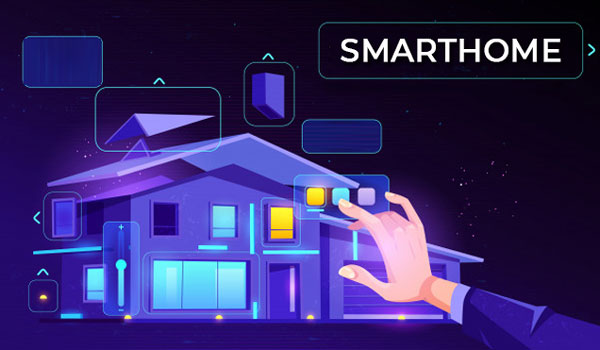
\includegraphics[scale=0.6]{img/smartHome.jpg}
%     \caption{Smart Home}
% \end{figure}
\newpage
\section{Requirement}
\subsection{Functional Requirement}
\subsubsection{Internet of things aspect}
\begin{itemize}
    
    \item Maintain ideal climatic conditions including temperature, venting, and lighting via different means: manually, automatically or periodically by schedule.
    \item Report issues that need manual intervention
    \item Provide live climate reports to the user via some form of display (graph view and log view).
    \item Periodically remind user to tend to manual tasks
\end{itemize}
\subsubsection{Web application aspect}
\begin{itemize}
    \item Allows users to check housing in a specific way, such as humidity, temperature, light
    \item Allows users to turn on or turn off devices such as fans, lights.
    \item Real-time display of temperature and related factors
    \item Statistical analysis and reports on the system’s condition and performance.
\end{itemize}
\subsection{Non-Functional Requirement}
\subsubsection{Internet of things aspect}
\begin{itemize}
    \item Run 24/7 with minimal scheduled downtime and preferably no unscheduled downtime.
    \item Device handling packaged in one or more MQTT server(s).
    \item The IoT system must be easily maintained, updated, and managed every year with minimal disruption to existing systems and processes.
    \item The IoT system should be able to handle a large number of devices and data streams as the number of connected devices increases over time, at least 10 devices.
    \item Actuator delay time should be no more than five seconds.
    \item Persistently log historical readings for diagnostic purposes that keep tracks of the system’s status over at least 200 days.
    \item Scalable and efficient database system that has a capacity of at least 400MB.
\end{itemize}
\subsubsection{Web application aspect}
\begin{itemize}
    \item The system must ensure working correctly 24/7.
    \item Intuitive interface, comfortable to see, suitable for all users.
    \item Users can use fluently after 15 minutes of learning.
    \item Data transfers and queries between web application and devices must be at maximum 2 seconds for each action.
    \item Application can support multi-platforms.
    \item The system must be designed with a strong security framework to prevent unauthorized access, data breaches, and cyber-attacks.
\end{itemize}
\section{Devices}
\subsection{Input devices}
\subsubsection {\textit{Infrared sensor}}
\begin{itemize}
    \item Characteristics: It can detect an obstacle effectively.
    \item Usage: Used to detect motion in the room and notify high -temperature equipment exceeding the permitted ink
\end{itemize}
\subsubsection {\textit{DHT20 sensor}}
\begin{itemize}
    \item Characteristics: Measure humidity(20\% - 90\% RH) and temperature(0 ~ 50 °C).
    \item Usage: Environmental control in the house.
\end{itemize}
\subsubsection {\textit{Light sensor}}
\begin{itemize}
    \item Characteristics: Check the light condition.
    \item Usage: Light sensors can be used to automatically turn on or off lights based on the amount of ambient light in a room or outdoor area.
\end{itemize}
\subsubsection {\textit{USB switch}}
\begin{itemize}
    \item Characteristics: Allows multiple USB devices to be shared between two or more computers. 
    
    \item Usage: Turn on and off the power supply for electronic devices via the USB port.
\end{itemize}
\subsubsection {\textit{Yolo bit}}
\begin{itemize}
    \item Characteristics: This is the central control circuit.
    \item Usage: Handle communication between server and devices.
\end{itemize}
\subsubsection {\textit{Expansion circuit}}
\begin{itemize}
    \item Characteristics: Support connection.
    \item Usage: Help Yolo bit add more ports connection.
\end{itemize}

\subsection{Output devices}
\subsubsection {\textit{Buzzer}}
\begin{itemize}
    \item Characteristics: Equipped with sound generating components that can be controlled by voltage input.
    \item Usage: Notify the user of the event taking place.
\end{itemize}
\subsubsection {\textit{LCD 16x2}}
\begin{itemize}
    \item Characteristics: Communicate with Yolo bit.
    \item Usage: Display the time and other notification.
\end{itemize}
\subsubsection {\textit{Led RGB}}
\begin{itemize}
    \item Characteristics: Produce a Wide Range of Colors by Varying the Intensity of Each Color Channel.
    \item Usage: Lighting at night.
\end{itemize}
\section{Use-case Details}
\section{Database Overview}
\section{Technical Diagram}
\section{Architecture design}
\subsection{Client Server Architecture}
\subsection{System design: factory method pattern}
\section{Mockup User Interface}
    \begin{lstlisting}
import React from 'react'

import '../css_pages/Login.css'

function Login(){
    const USER_NAME = "ADMIN";
    const PASSWORD = "ADMIN";
    
    return(
        <form>
            <div className = "login-form">
                <h2>Login</h2>
                <div className= "form-group">
                    <label htmlFor="email">Email</label>
                    <input type="text" name = "email" id = "email" />
                </div>
                <div className="form-group">
                    <label htmlFor="password">Password</label>
                    <input type="text" name="password" id="password" />
                </div>
                <input className='login-button' type="submit" value= "Login" />
            </div>
        </form>
    )
}

export default Login;
    \end{lstlisting}
\end{document}

